\documentclass[class=jsarticle, crop=false, dvipdfmx, fleqn]{standalone}
\input{/Users/User/Documents/TeX/preamble/mypreamble}
\begin{document}
\section*{練習問題6-1}

\subsection*{(1)}
ノイズ(誤差項)$\varepsilon$が正規分布$N(0, 1)$に従うから,
最尤推定による解と最小二乗法による解は一致する。
scipy.optimize.leastsqを用いて最小二乗法による解を求めると,
\begin{equation}
a = 1.059
\end{equation}
と求まる。


\subsection*{(2)}
$a$の事前分布が$p(a) = N(1, 0.09)$であるとする。
ノイズの分散を${\sigma_\mathrm{e}}^2$,
$a$の平均を$\mu_a$,分散を${\sigma_a}^2$とする。

まず一般の線形回帰問題を考える。
以下のようなモデルのMAP推定を行う。
\begin{align}
& y = \bm{a^T X} + \bm{\varepsilon} \\
& \epsilon \sim N(0, {\sigma_\mathrm{e}}^2) \\
& p(\bm{a}) = N(\mu_a, {\sigma_a}^2)
\end{align}
対数尤度関数は以下のようになる。
\begin{align*}
LL(\bm{a}, {\sigma_\mathrm{e}}^2)
	& = \log \prod_{i=1}^{N} p(y_i | \bm{x}_i, \bm{a}, {\sigma_\mathrm{e}}^2) p(\bm{a}) \\
	& = \sum_{i=1}^{N} \log\qty{ p(y_i | \bm{x}_i, \bm{a}, {\sigma_\mathrm{e}}^2) p(\bm{a}) } \\
	& = \sum_{i=1}^{N} \log\qty{ \frac{1}{\sqrt{2 \pi {\sigma_\mathrm{e}}^2}} \exp\qty(-\frac{(\epsilon_i)^2}{2{\sigma_\mathrm{e}}^2}) \cdot
		\frac{1}{\sqrt{2 \pi {\sigma_a}^2}} \exp\qty(-\frac{(a_i - \mu_a)^2}{2{\sigma_a}^2}) } \\
	& = \sum_{i=1}^{N} \qty{ - \frac{1}{2{\sigma_\mathrm{e}}^2} {\varepsilon_i}^2 - \frac{1}{2{\sigma_a}^2} (a_i - \mu_a)^2} - \frac{N}{2} \qty{\log(2 \pi {\sigma_\mathrm{e}}^2) + \log(2 \pi {\sigma_a}^2)} \\
	& = -\frac{1}{2{\sigma_\mathrm{e}}^2} \qty(\|\bm{\varepsilon}\|^2 + \frac{{\sigma_\mathrm{e}}^2}{{\sigma_a}^2} \|(\bm{a} - \mu_a)\|^2) - N \log(2 \pi \sigma_\mathrm{e} \sigma_a) \\
	& = -\frac{1}{2{\sigma_\mathrm{e}}^2} \qty(\|\bm{y - Xa}\|^2 + \frac{{\sigma_\mathrm{e}}^2}{{\sigma_a}^2} \|(\bm{a} - \mu_a)\|^2) - N \log(2 \pi \sigma_\mathrm{e} \sigma_a)
\end{align*}
よって,
\begin{equation}
LL(\bm{a}, {\sigma_\mathrm{e}}^2) \text{が最大}
\quad \Leftrightarrow \quad
\|\bm{y - Xa}\|^2 + ({\sigma_\mathrm{e}}^2/{\sigma_a}^2) \|(\bm{a} - \mu_a)\|^2 \text{が最小}
\end{equation}
ここで,
\begin{equation}
\lambda = \frac{{\sigma_\mathrm{e}}^2}{{\sigma_a}^2}
\end{equation}
とおくと,
$\|\bm{y - Xa}\|^2 + \lambda \|(\bm{a} - \mu_a)\|^2$を最小にすればよいことがわかる。

ここで,配布資料より,
\begin{equation}
\begin{split}
\log p(\bm{a} | \bm{X}, \bm{y}, \sigma^2) & = -\frac{1}{2 \sigma^2} \|\bm{y - Xa}\|^2 - \frac{\lambda}{2\sigma^2} \|\bm{a}\|^2 + \mathrm{Const.} \\
	& = -\frac{1}{2 \sigma^2} \qty(\|\bm{y - Xa}\|^2 + \lambda \|\bm{a}\|^2) + \mathrm{Const.}
\end{split}
\end{equation}
を最大にする$\bm{a}$は,
\begin{equation}
\hat{\bm{a}}_\mathrm{MAP} = \qty(\bm{X}^T \bm{X} + \lambda \bm{I})^{-1} \qty(\bm{X}^T \bm{y})
\end{equation}
となることがわかる。
よって,
\begin{equation}
\bm{b} = \bm{a} - \mu_a, \quad
\bm{z} = \bm{y} - \mu_a \bm{X}
\end{equation}
と変換すると,
\begin{equation}
\|\bm{y - Xa}\|^2 + \lambda \|(\bm{a} - \mu_a)\|^2 = \|\bm{z - Xb}\|^2 + \lambda \|\bm{b}\|
\end{equation}
を最小にすればよいから,その解は,
\begin{equation}
\hat{\bm{b}}_\mathrm{MAP} = \qty(\bm{X}^T \bm{X} + \lambda \bm{I})^{-1} \qty(\bm{X}^T \bm{z})
\end{equation}
結局,対数尤度関数$LL(\bm{a}, {\sigma_\mathrm{e}}^2)$を最大にする$\bm{a}$は,
\begin{equation}
\begin{split}
\hat{\bm{a}}_\mathrm{MAP} & = \hat{\bm{b}}_\mathrm{MAP} + \mu_a \\
	& = \qty(\bm{X}^T \bm{X} + \lambda \bm{I})^{-1} \qty(\bm{X}^T \bm{z}) + \mu_a \\
	& = \qty(\bm{X}^T \bm{X} + \lambda \bm{I})^{-1} \qty(\bm{X}^T \bm{y} - \mu_a \bm{X}^T \bm{X}) + \mu_a
\end{split}
\label{eq:q6-1_a_MAP}
\end{equation}
と表せる。

式(\ref{eq:q6-1_a_MAP})に,
\begin{align}
& \mu_a = 1 \\
& \lambda = \frac{{\sigma_\mathrm{e}}^2}{{\sigma_a}^2} = \frac{1}{0.09} = \frac{100}{9} \\
\end{align}
と$\bm{X},\ \bm{y}$を代入すると,
\begin{equation}
a = 1.028
\end{equation}
を得る。

以下にMLE,MAP推定それぞれの結果のグラフを示した。

\begin{figure}[H]
\centering
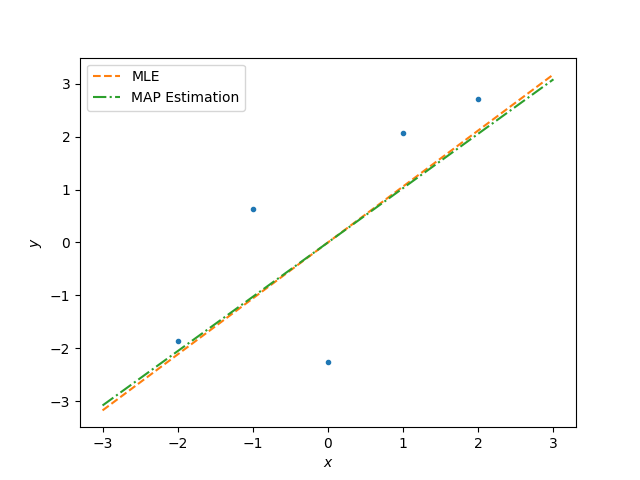
\includegraphics[clip, width=12cm]{../figures/q_6_1}
\caption{【練習問題6-1】 MLEとMAP推定による線形回帰のグラフ}
\label{fig:q6-1_MLE_MAP_graph}
\end{figure}


\end{document}